\documentclass[10pt,twocolumn]{article}
\usepackage[margin=0.85in,top=0.9in]{geometry}
\usepackage{amsmath,amssymb,bm}
\usepackage{graphicx}
\usepackage{booktabs}
\usepackage{siunitx}
\usepackage{microtype}
\usepackage{hyperref}
\usepackage[numbers,sort&compress]{natbib}
\usepackage{xcolor}
\hypersetup{colorlinks,linkcolor=blue!60!black,citecolor=blue!60!black,urlcolor=blue!60!black}
\graphicspath{{../figures/}}
\sisetup{detect-all}

\newcommand{\btheta}{\bm{\theta}}
\newcommand{\bx}{\mathbf{x}}
\newcommand{\expval}[1]{\langle #1 \rangle}

\title{\vspace{-1.2em}Bayesian-Optimized Variational Quantum Circuits\\
on a Classification Task:\\
\large A Comparison with Classical Neural Networks}
\author{Jialun Li \and Juan Vera}
\date{\normalsize \today}

\begin{document}
\maketitle

\begin{abstract}
We train a two-qubit, 24-parameter variational quantum circuit (VQC) to classify
the two-moons dataset using Bayesian optimization (BO), a gradient-free method that
treats the circuit loss as a black box, and compare it with classical neural
networks trained by backpropagation. The circuit uses data re-uploading so that its
output is a trainable Fourier series in the inputs. We find that Gaussian-process BO
over all 24 parameters at once is no better than random search (\SI{79}{\percent}
test accuracy), but that running BO on one circuit layer at a time recovers
\SI{93}{\percent}, and a short derivative-free local polish brings the circuit to
$\SI{96.0}{\percent}\pm\SI{0.0}{\percent}$ over three seeds, on par with a
17-parameter multilayer perceptron (\SI{95.3}{\percent}) and a 1185-parameter one
(\SI{96.0}{\percent}). The trained circuit loses under one point of accuracy when
read out with 256 measurement shots. We also report that on an exact simulator the
local optimizer COBYLA alone matches the BO pipeline, so the case for BO in this
setting rests on the noisy-evaluation regime that our experiment does not probe.
Code, results and a live terminal dashboard are provided.
\end{abstract}

\section{Introduction}

Variational quantum circuits are parametrized unitaries whose expectation values
serve as a machine-learning model; a classical optimizer adjusts the parameters to
minimize a loss \citep{cerezo2021vqa}. On hardware, gradients are available only
through the parameter-shift rule \citep{schuld2019gradients}, which costs two extra
circuit executions per parameter per data point, and every execution is a noisy
estimate. This makes sample-efficient, gradient-free optimizers attractive, and
Bayesian optimization \citep{frazier2018bo,shahriari2016bo} is the canonical such
method: it fits a probabilistic surrogate to all loss values seen so far and
chooses each new query to maximize expected improvement.

This project asks two concrete questions on a toy task small enough to simulate
exactly:
\begin{enumerate}\setlength\itemsep{0pt}
  \item Can a BO-trained VQC reach the accuracy of a classical neural network with a
        comparable number of parameters?
  \item Does BO actually help, compared with random search and with a simpler
        derivative-free local optimizer at the same evaluation budget?
\end{enumerate}

\section{Model}

\paragraph{Task.} Two interleaving moons (\texttt{sklearn.make\_moons}, noise
0.2), $N{=}300$ points, split 200/100 into train/test, features scaled to
$[-1,1]^2$, labels $y\in\{-1,+1\}$ (Fig.~\ref{fig:data}). A linear classifier
reaches about \SI{84}{\percent}; the rest requires a curved boundary.

\begin{figure}[t]
  \centering
  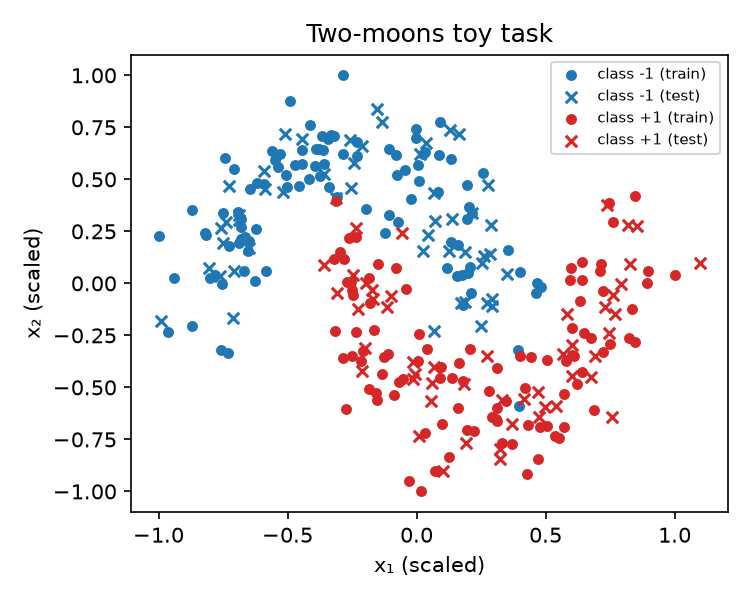
\includegraphics[width=0.78\linewidth]{dataset.png}
  \caption{The two-moons task after scaling. Dots are training points, crosses
  test points.}
  \label{fig:data}
\end{figure}

\paragraph{Circuit.} We use a two-qubit data re-uploading circuit
\citep{perezsalinas2020reuploading} with $L{=}4$ layers. Layer $\ell$ applies
\begin{equation}
U_\ell(\bx;\btheta)=\mathrm{CZ}\cdot\!\bigotimes_{q=1}^{2}\!R_Y(\beta_{\ell q})R_Z(\alpha_{\ell q})
\cdot\!\bigotimes_{q=1}^{2}\!R_Y(w_{\ell q}\,x_q),
\end{equation}
i.e.\ feature $x_q$ is encoded on qubit $q$ with a \emph{trainable} scale
$w_{\ell q}$, followed by a trainable rotation and a CZ entangler. Six parameters
per layer give $P{=}24$ in total. The output is
\begin{equation}
f(\bx;\btheta)=\expval{00|\,U^\dagger (Z\otimes I)\,U\,|00}\in[-1,1],
\qquad \hat y=\operatorname{sign} f,
\end{equation}
and the training loss is the mean squared error
$\mathcal L(\btheta)=\frac1N\sum_i\big(f(\bx_i;\btheta)-y_i\big)^2$.

Because $R_Y(wx)=\cos\frac{wx}{2}I-i\sin\frac{wx}{2}Y$, every matrix element of an
encoding gate is a combination of $e^{\pm iwx/2}$, and $f$ is a finite Fourier
series in $\bx$ whose frequencies are signed sums of the $w_{\ell q}$
\citep{schuld2021fourier}. The rotation angles set the Fourier coefficients and the
trainable scales set the spectrum; each re-upload adds frequencies. A single encoding
layer would give one frequency per feature, far too smooth for the moons.

\paragraph{Simulation.} The loss is evaluated exactly with Qiskit's
\texttt{StatevectorEstimator} \citep{qiskit2024}, batched over the 200 training
points. After training we also re-evaluate the best circuit with 256 shots per
point on \texttt{AerSimulator}, where $\hat f=\frac1S\sum_b(-1)^{b_0}n_b$ has
standard error $\le 1/16$.

\section{Optimizers}

All circuit optimizers see only scalar loss values. Budgets are in loss
evaluations, each of which runs 200 circuits.

\paragraph{Full-space BO.} \texttt{gp\_minimize} from scikit-optimize
\citep{skopt}: a Gaussian process with an ARD Mat\'ern-5/2 kernel over
$[-\pi,\pi]^{24}$, 25 Latin-hypercube initial points, then 125 points chosen by
Expected Improvement,
\begin{equation}
\mathrm{EI}(\btheta)=(\mathcal L^*-\mu)\,\Phi(z)+\sigma\,\varphi(z),\quad
z=\tfrac{\mathcal L^*-\mu(\btheta)}{\sigma(\btheta)} .
\end{equation}
The budget is capped at 150 because GP fitting costs $O(t^3)$ in the number of
observations.

\paragraph{Block-coordinate BO.} The same optimizer applied to one layer's six
parameters at a time with the other 18 frozen, 40 calls per block with the incumbent
supplied as a known point, cycling through the four layers for three sweeps (481
evaluations). Updates are accepted only on improvement, so the loss is monotone.
This is in the spirit of layerwise training \citep{skolik2021layerwise} and keeps
the GP in the dimensionality range where it is informative.

\paragraph{Block BO + polish (main pipeline).} Block BO followed by 150 iterations
of COBYLA \citep{powell1994cobyla}, a derivative-free trust-region method that fits a
linear model through $P{+}1$ points, started from the block-BO solution with trust
radius $0.2$. Total 631 evaluations.

\paragraph{Controls.} Random search over $[-\pi,\pi]^{24}$ and COBYLA from a random
start, each with 631 evaluations.

\paragraph{Classical baselines.} Logistic regression (3 parameters); a 2--4--1
multilayer perceptron with $\tanh$ units (17 parameters, the parameter-matched
comparison); and a 2--32--32--1 MLP (1185 parameters). All are trained with L-BFGS on
the logistic loss in scikit-learn \citep{sklearn}.

Every method is run for three seeds, which change the data split, the BO initial
design and the random starts.

\section{Results}

\begin{table*}[t]
  \centering
  \caption{Mean $\pm$ standard deviation over three seeds. Evaluations are
  circuit-loss evaluations (200 circuits each). The main pipeline re-evaluated
  with 256 measurement shots per point scores $0.953\pm0.005$ on the test set.}
  \label{tab:results}
  \begin{tabular}{llcccc}
    \toprule
    Model & Optimizer & Params & Train acc & Test acc & Evals \\
    \midrule
    VQC & Full-space BO (GP, EI)          & 24 & $0.818\pm0.019$ & $0.790\pm0.014$ & 150 \\
    VQC & Block-coordinate BO              & 24 & $0.938\pm0.027$ & $0.933\pm0.039$ & 481 \\
    VQC & \textbf{Block BO + COBYLA polish} & 24 & $0.960\pm0.007$ & $\mathbf{0.960\pm0.000}$ & 631 \\
    VQC & Random search                    & 24 & $0.812\pm0.017$ & $0.790\pm0.029$ & 631 \\
    VQC & COBYLA (random init)             & 24 & $0.972\pm0.008$ & $0.963\pm0.005$ & 631 \\
    \midrule
    Logistic regression & L-BFGS           & 3    & $0.855\pm0.004$ & $0.843\pm0.017$ & -- \\
    MLP 2--4--1         & L-BFGS           & 17   & $0.985\pm0.004$ & $0.953\pm0.017$ & -- \\
    MLP 2--32--32--1    & L-BFGS           & 1185 & $1.000\pm0.000$ & $0.960\pm0.016$ & -- \\
    \bottomrule
  \end{tabular}
\end{table*}

\begin{figure}[t]
  \centering
  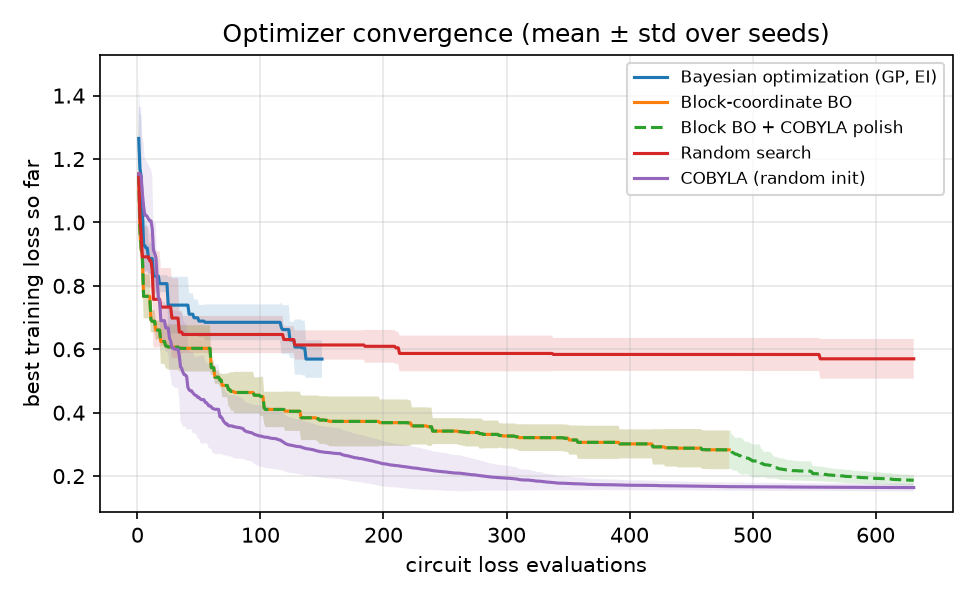
\includegraphics[width=\linewidth]{convergence.png}
  \caption{Best training loss versus loss evaluations, mean $\pm$ std over seeds.
  Full-space BO (blue) overlaps random search (red). Block BO (orange, hidden under
  the dashed green curve for its first 481 evaluations) descends steadily; the
  COBYLA polish (dashed) continues from it. COBYLA from a random start (purple)
  converges fastest.}
  \label{fig:conv}
\end{figure}

\begin{figure*}[t]
  \centering
  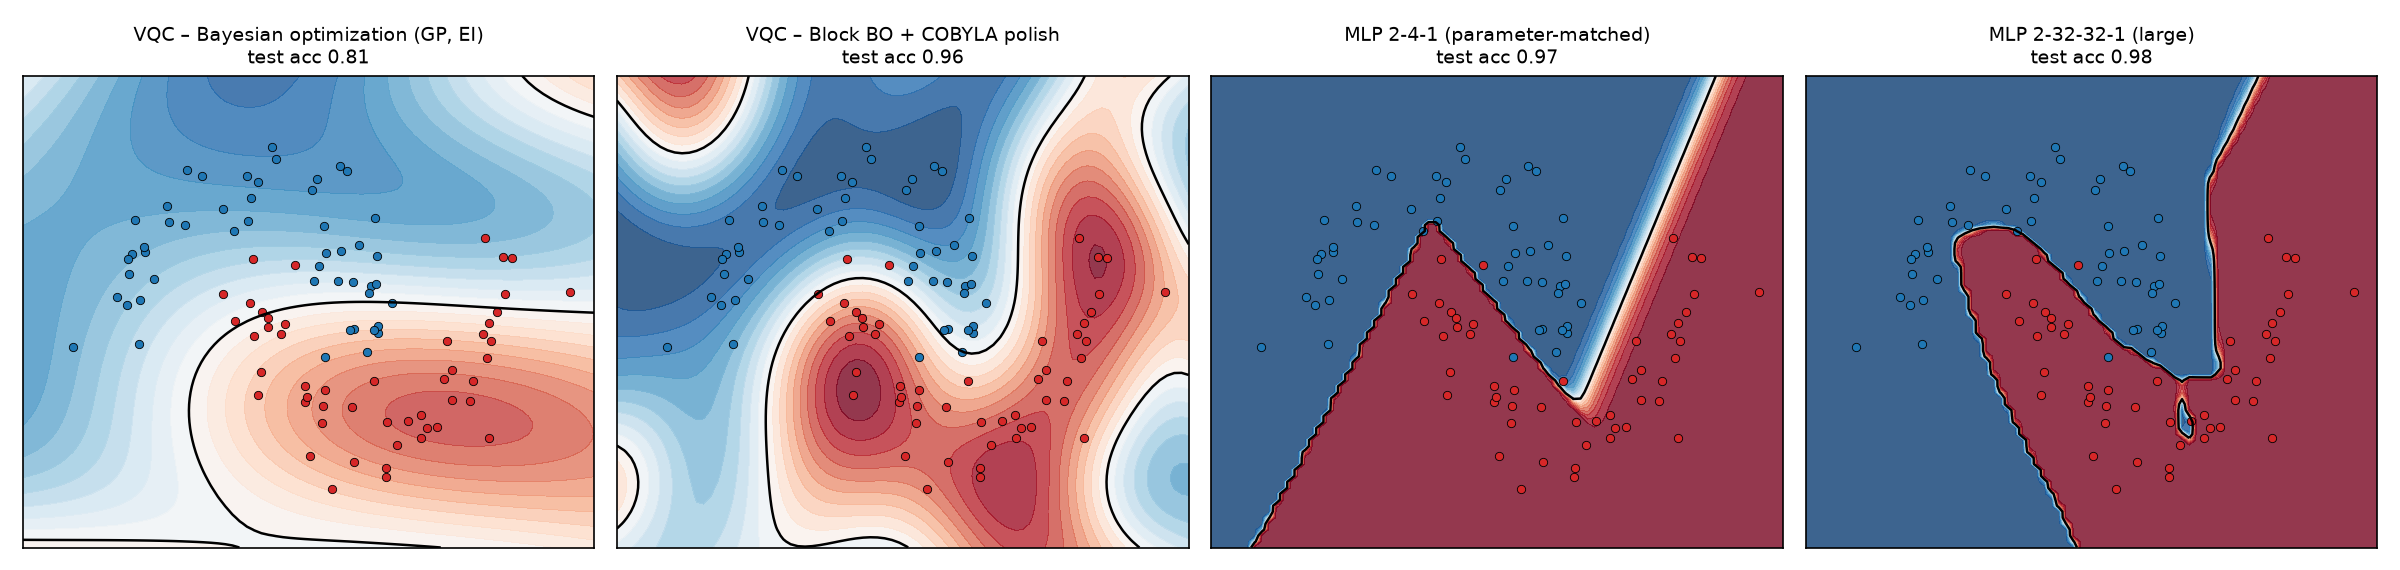
\includegraphics[width=\textwidth]{decision_boundaries.png}
  \caption{Decision functions on seed 0 with test points overlaid. Left to right:
  VQC after full-space BO; VQC after block BO + polish; parameter-matched MLP; large
  MLP. The black contour is the decision boundary. The VQC boundary is smooth and
  periodic, the MLP boundary piecewise-sigmoidal.}
  \label{fig:bound}
\end{figure*}

Table~\ref{tab:results} and Figs.~\ref{fig:conv}--\ref{fig:bound} summarize the
experiment.

\paragraph{The VQC matches the classical networks.} The main pipeline reaches
\SI{96.0}{\percent} test accuracy on every seed, equal to the 1185-parameter MLP and
slightly above the parameter-matched MLP. With 100 test points a difference of one
or two points is within noise, so the fair reading is parity. The classical models
fit the training set more tightly (\SIrange{98.5}{100}{\percent} versus
\SI{96}{\percent}), so the VQC is the less expressive model and generalizes about
as well.

\paragraph{Finite shots cost little.} Reading out with 256 shots instead of exact
expectation values drops test accuracy from $0.960$ to $0.953\pm0.005$: the trained
boundary is not relying on margins smaller than the shot-noise scale.

\paragraph{Full-space BO fails at $P{=}24$.} Its test accuracy ($0.790$) is
identical to random search and its convergence curve overlaps it
(Fig.~\ref{fig:conv}). During development, more calls (200, 300), other
acquisition functions (LCB, hedge) and larger initial designs did not change this.
A GP conditioned on 150 points in a 24-dimensional periodic landscape with many
local minima has a posterior close to its prior almost everywhere, so EI is nearly
flat and its maximizer is effectively a random draw. This is the well-known
dimensionality ceiling of GP-based BO, and VQC parameter counts cross it quickly.

\paragraph{Block-coordinate BO recovers most of the gap.} Restricting each BO run to
six parameters brings the loss from $0.57$ to $0.28$ and accuracy to
\SI{93}{\percent}, with the same optimizer and no gradients. It is seed-sensitive
(\SIrange{88}{97}{\percent}), as coordinate descent can stop at a point that is
optimal per block but not jointly; the per-sweep logs show improvements becoming rare
after the second sweep.

\paragraph{A short local polish closes the rest.} 150 COBYLA iterations from the
block-BO solution remove the seed sensitivity entirely. This is the usual
global-then-local pattern: BO locates a basin, a local method descends it.

\paragraph{The control is uncomfortable.} COBYLA from a random start, with the same
631 evaluations, reaches $0.963\pm0.005$ and converges faster than the pipeline. On a
noiseless simulator the landscape is smooth enough that following the local slope
already works, and the global search that BO is meant to provide bought nothing
here. BO's expected advantages, robustness to noisy evaluations and sample
efficiency when each evaluation is very costly, are precisely the conditions this
experiment does not create.

\paragraph{Model shapes differ.} Fig.~\ref{fig:bound} shows the structural contrast
between the model families. The MLP boundary is a few straight segments joined by
bends, a sum of sigmoidal ridges. The VQC boundary is smooth and repeats outside the
data region because $f$ is a band-limited Fourier series in the inputs. Both fit the
moons; they extrapolate very differently.

\section{Discussion and limitations}

Nothing here is a quantum advantage, nor could it be: a two-qubit state is a
four-component vector and the whole model is a small classical linear-algebra
computation. The argument for VQCs rests on regimes where the state space is too
large to simulate, which a two-qubit toy cannot reach. What the experiment does
establish is that a gradient-free optimizer can train such a model to classical
parity, and it characterizes which gradient-free optimizer.

The main limitation is the noiseless loss. With shot noise in the training loss,
COBYLA's linear interpolation is corrupted while a GP with a noise term should remain
reliable; that experiment, along with smaller budgets, is the natural next step and
the one that could make BO's contribution positive rather than neutral. A second
limitation is scale: at larger qubit counts barren plateaus
\citep{mcclean2018barren} flatten the landscape and change the picture for every
optimizer. Finally, the 100-point test set bounds how finely the methods can be
ranked.

\section{Conclusion}

A 2-qubit, 24-parameter re-uploading circuit trained without gradients reaches
\SI{96}{\percent} test accuracy on two-moons, on par with classical MLPs with 17 and
1185 parameters. Gaussian-process Bayesian optimization over all parameters at once
fails at this dimensionality; restricting it to one layer at a time makes it work,
and a short local polish makes it reliable. On an exact simulator the simpler
COBYLA optimizer is equally good, so the case for BO must be made in the noisy or
very-expensive-evaluation regime.

\paragraph{Reproducibility.} Code, per-seed results and figures are in the project
repository. \texttt{run\_experiment.py --seed k} reproduces one seed in about five
minutes; \texttt{aggregate.py} builds the table and figures; \texttt{train\_live.py}
and \texttt{compare\_live.py} show training live in the terminal.

\bibliographystyle{unsrtnat}
\bibliography{refs}

\end{document}
